\chapter{Herramientas}
\section{Raspberry Pi}

Raspberry Pi es una computadora de placa de bajo costo que corre GNU/Linux y otros sistemas operativos. Existen dos modelos el A y B, el modelo B tiene la revisi�n 1 y 2, y adem�s de una nueva versi�n que es B+.
%TODO aumentar algo mas
\subsection{Componentes}
\begin{itemize}
\item Broadcom BCM2835, SoC que contiene memoria, microprocesador y procesador gr�fico.
\item Conector GPIO (Entradas y salidas de prop�sito general).
\item Conector salida de video compuesto
\item Conector salida de video HDMI
\item LEDs de actividad de LAN y Power
\item Conector de salida de audio
\item Conector microusb para alimentaci�n
\item Circuito integrado para LAN
\item Conectores de expansi�n (para c�mara de video y salida de video)
\item Conectores USB
\item Conector RJ45 para Ethernet
\item Reguladores de voltaje de 1.8v, 2.8v y 3.3v 
\end{itemize}

\begin{figure}
  \centering
    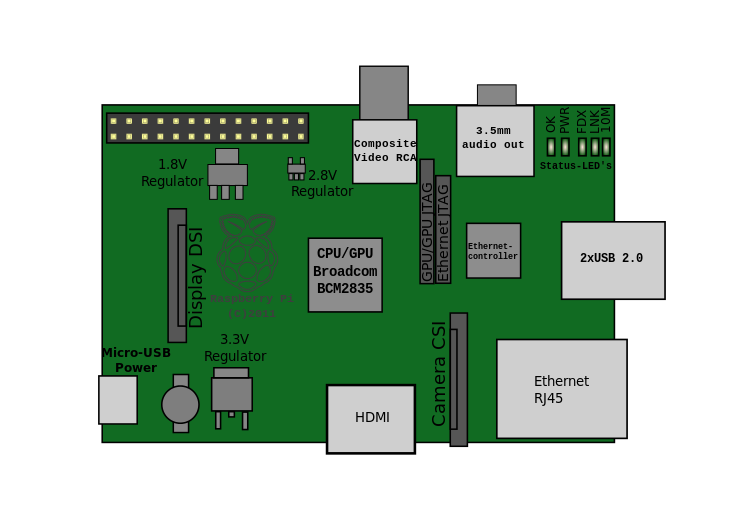
\includegraphics[width=0.5\textwidth]{raspi_pcb}
  \caption{Ubicaci�n de los componentes de Raspberry Pi. \cite{raspberry_pi_wiki}}
  \label{fig:raspi_pcb}
\end{figure}

\begin{table}
\centering
  \begin{tabular}{r r r r}
\textbf{Pin} & \textbf{Descripci�n} & \textbf{Pin} & \textbf{Descripci�n} \\
\hline
1 & \texttt{3.3v} & 2 & \texttt{5v} \\
3 & \texttt{SDA0*} & 4 & \texttt{5v} \\
5 & \texttt{SCL0*} & 6 & \texttt{GND} \\
7 &  \texttt{GPIO\_GCLK} & 8 & \texttt{TXD0*} \\
9 &  \texttt{GND} & 10 & \texttt{RXD0*} \\
11 &  \texttt{GPIO\_GEN0} & 12 & \texttt{GPIO\_GEN1} \\
13 &  \texttt{GPIO\_GEN2} & 14 & \texttt{GND} \\
15 &  \texttt{GPIO\_GEN3} & 16 & \texttt{GPIO\_GEN4} \\
17 &  \texttt{3.3v} & 18 & \texttt{GPIO\_GEN5} \\
19 &  \texttt{SPI\_MOSI*} & 20 & \texttt{GND} \\
21 &  \texttt{SPI\_MISO*} & 22 & \texttt{GPIO\_GEN6} \\
23 &  \texttt{SPI\_SCLK*} & 24 & \texttt{SPI\_CEO\_N*} \\
25 &  \texttt{GND} & 26 & \texttt{SPI\_CE1\_N*} \\
  \end{tabular}
  \caption{Descripci�n de los pines de GPIO}
  \label{table:gpio_descr}
\end{table}

\section{Conclusiones}

blah blah.
